\documentclass{article}
\usepackage{booktabs}
\usepackage{multirow}
\usepackage{caption}
\usepackage{geometry}
\usepackage{xcolor}
\usepackage{colortbl}
\usepackage{makecell}
\usepackage{setspace}
\usepackage{pdflscape}
\usepackage{tikz}
\usepackage{hyperref}
\usepackage{parskip}
\usetikzlibrary{shapes.geometric, arrows, positioning, fit, calc}
\definecolor{lightblue}{RGB}{173,216,230}
\tikzset{
    process/.style={rectangle, minimum width=4cm, minimum height=1cm,
        text centered, draw=black, thick, text width=3.8cm, align=center},
    excluded/.style={rectangle, minimum width=3cm, minimum height=1cm,
        text centered, draw=black, thick, text width=3.8cm, align=center},
    phaselabel/.style={rectangle, fill=lightblue, minimum width=2.5cm,
        minimum height=1cm, text centered, draw=black, thick, rotate=90,
        text width=2.3cm, align=center},
    arrow/.style={thick, ->, >=stealth}
}
\renewcommand\theadfont{\normalfont}
\renewcommand\theadgape{}
\geometry{margin=1in}

% \pctN{pct}{N} prints pct then (N) in grey, both at ambient font size
\newcommand{\pctN}[2]{#1 {\textcolor{gray}{(#2)}}}

% Paragraph outline headers (delete before submission)
\newcommand{\outline}[1]{\paragraph{\textit{[#1]}}\mbox{}\\}

\begin{document}
\doublespacing

% ==================== TITLE PAGE ====================
\title{Ignoring clustering or restricted randomization is common in NHLBI-funded trials with clusters, and mirrors patterns seen in NCI-funded trials}
\author{Deborah H. Glueck and Keith E. Muller}
\date{}
\maketitle

% ==================== ABSTRACT ====================
\begin{abstract}
\subsection*{Background/Aims}
[State the problem. State the aims. Reference NCI companion paper.]

\subsection*{Methods}
[NHLBI search. Inclusion criteria. Comparison methods.]

\subsection*{Results}
[Key numbers. CMH and Fisher results.]

\subsection*{Conclusions}
[NHLBI vs NCI. Implications.]
\end{abstract}

\newpage

% ==================== INTRODUCTION ====================
\section{Introduction}

\outline{Background: clustering and restricted randomization}

\outline{Consequences of ignoring: Type I error and power}

\outline{Prior systematic reviews: high rates of incorrect analyses}

\outline{NCI companion paper: motivation for NHLBI comparison}

\outline{Aims}

% ==================== METHODS ====================
\section{Methods}

\subsection{Systematic review}

\outline{PRISMA~\cite{page_prisma_2021} and search strategy}

\outline{Exclusion criteria}

\outline{Review process: two reviewers, consensus conference}

\outline{Classification of incorrect analyses}

\subsection{Statistical comparisons between NCI and NHLBI}

\outline{Table~\ref{tab:PowerStatAnalysis}: CMH test}

\outline{Tables~\ref{tab:IgnoredPower} and~\ref{tab:IgnoredData}: CMH test across all three strata}

\outline{Software}

% ==================== RESULTS ====================
\section{Results}

\subsection{Systematic review results}

\outline{PRISMA: how many identified, screened, included (Figure~\ref{fig:PRISMA}~\cite{page_prisma_2021})}

\outline{Overall rates: correct/incorrect. CMH result (Table~\ref{tab:PowerStatAnalysis})}

\outline{What was ignored in power analyses (Table~\ref{tab:IgnoredPower}). CMH result.}

\outline{What was ignored in data analyses (Table~\ref{tab:IgnoredData}). CMH result.}

% ==================== DISCUSSION ====================
\section{Discussion}

\outline{Summary: NHLBI vs NCI}

\outline{Consistency with prior literature}

\outline{Policy implications}

\outline{Strengths: PRISMA~\cite{page_prisma_2021}. Novel NCI vs NHLBI comparison.}

\outline{Limitations}

% ==================== CONCLUSIONS ====================
\section{Conclusions}

\outline{Restate main finding. Call to action.}

% ==================== ACKNOWLEDGMENTS ====================
\section*{Acknowledgments}
The inception of this work was supported by R01GM121081 from the National Institute of General Medical Sciences of the United States National Institutes of Health to the University of Colorado Denver (Dana Dabelea, Deborah H. Glueck, Keith E. Muller MPI). The opinions, findings, and conclusions of the authors are their own and do not necessarily reflect the official views, policies, or positions of the National Institutes of Health or the United States government.

% ==================== REFERENCES ====================
\bibliographystyle{SageV}
\bibliography{references}

% ==================== TABLES ====================
\clearpage

% ==================== TABLE 1: PowerStatAnalysis ====================
\begin{table}[p]
\normalsize\centering
\captionsetup{width=\linewidth}
\caption{Correct and incorrect data and power analysis rates in systematic reviews of NCI (left) and NHLBI (right) trials with clusters. Values are percentages with counts in grey; $\mathcal{N}$ = 96 manuscripts reviewed for NCI-funded studies, $\mathcal{N}$ = xx manuscripts reviewed for NHLBI-funded studies.}
\label{tab:PowerStatAnalysis}
\setlength{\tabcolsep}{6pt}
\begin{minipage}[t]{0.42\linewidth}
\centering
\textbf{NCI-funded studies}\\[6pt]
\begin{tabular}{ll ccc}
\toprule
& & \multicolumn{2}{c}{\shortstack{Power or sample\\size analyses}} & \\
\cmidrule(lr){3-4}
& & Correct & Incorrect & Total \\
\midrule
\multirow{2}{*}{\shortstack{Data\\analyses}}
  & Correct   & \pctN{20.8}{20} & \pctN{11.5}{11} & \pctN{32.3}{31} \\[6pt]
  & Incorrect & \pctN{5.2}{5}   & \pctN{62.5}{60} & \pctN{67.7}{65} \\
\midrule
  & Total     & \pctN{26.0}{25} & \pctN{74.0}{71} & \pctN{100.0}{96} \\
\bottomrule
\end{tabular}
\end{minipage}
\hfill
\begin{minipage}[t]{0.42\linewidth}
\centering
\textbf{NHLBI-funded studies}\\[6pt]
\begin{tabular}{ll ccc}
\toprule
& & \multicolumn{2}{c}{\shortstack{Power or sample\\size analyses}} & \\
\cmidrule(lr){3-4}
& & Correct & Incorrect & Total \\
\midrule
\multirow{2}{*}{\shortstack{Data\\analyses}}
  & Correct   & & & \\[6pt]
  & Incorrect & & & \\
\midrule
  & Total     & & & \\
\bottomrule
\end{tabular}
\end{minipage}
\end{table}

\clearpage

% ==================== TABLE 2: IgnoredPower ====================
\begin{landscape}
\begin{table}[p]
\large\rmfamily\centering
\captionsetup{width=9in, font=large, labelfont=normalfont, textfont=normalfont}
\caption{Numbers and percentages [$\mathcal{N}$ (\%)] of manuscripts reviewed, cross-classified by design type and what was ignored in the power or sample size analyses, for NCI-funded and NHLBI-funded trials with clusters. Designs with clustering alone cannot have restricted randomization ignored; impossible cases are indicated by gray shading.}
\label{tab:IgnoredPower}
\setlength{\tabcolsep}{8pt}
\begin{tabular}{l ccc p{18pt} ccc}
\toprule
& \multicolumn{3}{c}{NCI-funded studies} & & \multicolumn{3}{c}{NHLBI-funded studies} \\
\cmidrule(lr){2-4}\cmidrule(lr){6-8}
& \makecell[t]{Ignored\\clustering\\alone}
& \makecell[t]{Ignored restricted\\randomization only}
& \makecell[t]{Ignored\\both}
&
& \makecell[t]{Ignored\\clustering\\alone}
& \makecell[t]{Ignored restricted\\randomization only}
& \makecell[t]{Ignored\\both} \\
\midrule
\shortstack[l]{Clustering\\alone}
  & \pctN{66.7}{20} & \cellcolor[gray]{0.85} & \cellcolor[gray]{0.85}
  & & & \cellcolor[gray]{0.85} & \cellcolor[gray]{0.85} \\[10pt]
\shortstack[l]{Both clustering\\and restricted\\randomization}
  & \pctN{0.0}{0} & \pctN{48.5}{32} & \pctN{28.8}{19}
  & & & & \\[10pt]
Total
  & \pctN{20.8}{20} & \pctN{33.3}{32} & \pctN{19.8}{19}
  & & & & \\
\bottomrule
\end{tabular}
\end{table}
\end{landscape}

\clearpage

% ==================== TABLE 3: IgnoredData ====================
\begin{landscape}
\begin{table}[p]
\large\rmfamily\centering
\captionsetup{width=9in, font=large, labelfont=normalfont, textfont=normalfont}
\caption{Numbers and percentages [$\mathcal{N}$ (\%)] of manuscripts reviewed, cross-classified by design type and what was ignored in the data analyses, for NCI-funded and NHLBI-funded trials with clusters. Designs with clustering alone cannot have restricted randomization ignored; impossible cases are indicated by gray shading.}
\label{tab:IgnoredData}
\setlength{\tabcolsep}{8pt}
\begin{tabular}{l ccc p{18pt} ccc}
\toprule
& \multicolumn{3}{c}{NCI-funded studies} & & \multicolumn{3}{c}{NHLBI-funded studies} \\
\cmidrule(lr){2-4}\cmidrule(lr){6-8}
& \makecell[t]{Ignored\\clustering\\alone}
& \makecell[t]{Ignored restricted\\randomization only}
& \makecell[t]{Ignored\\both}
&
& \makecell[t]{Ignored\\clustering\\alone}
& \makecell[t]{Ignored restricted\\randomization only}
& \makecell[t]{Ignored\\both} \\
\midrule
\shortstack[l]{Clustering\\alone}
  & \pctN{46.7}{14} & \cellcolor[gray]{0.85} & \cellcolor[gray]{0.85}
  & & & \cellcolor[gray]{0.85} & \cellcolor[gray]{0.85} \\[10pt]
\shortstack[l]{Both clustering\\and restricted\\randomization}
  & \pctN{0.0}{0} & \pctN{39.4}{26} & \pctN{37.9}{25}
  & & & & \\[10pt]
Total
  & \pctN{14.6}{14} & \pctN{27.1}{26} & \pctN{26.0}{25}
  & & & & \\
\bottomrule
\end{tabular}
\end{table}
\end{landscape}

\clearpage

% ==================== FIGURE 1: PRISMA ====================
\begin{figure}[p]
\centering
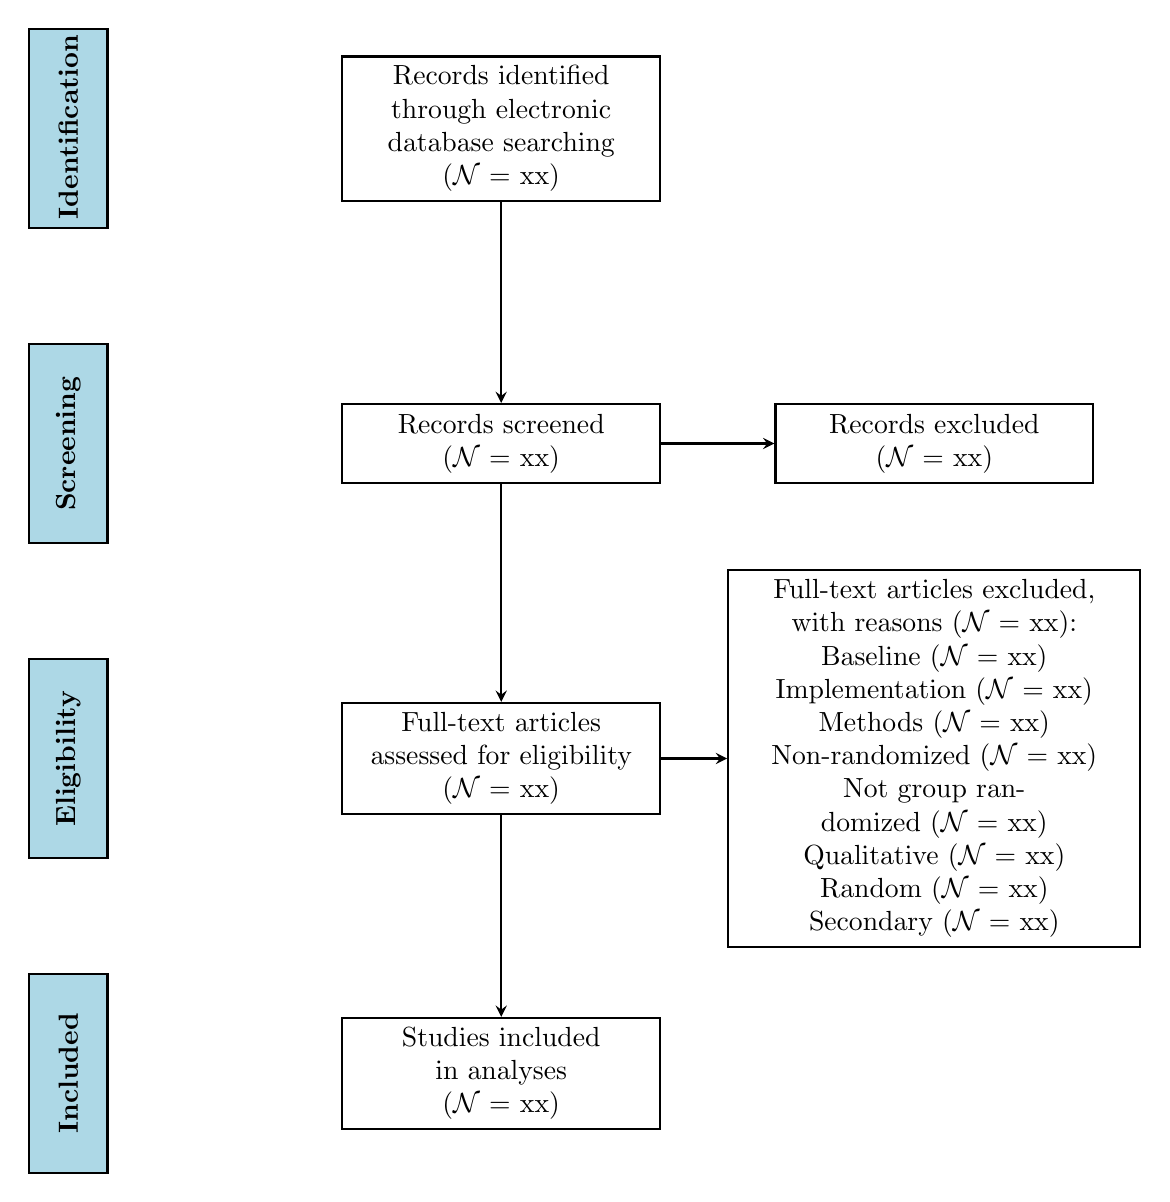
\begin{tikzpicture}[node distance=1.5cm]
\node[phaselabel] at (-5.5, 0)  {\textbf{Identification}};
\node[phaselabel] at (-5.5,-4)  {\textbf{Screening}};
\node[phaselabel] at (-5.5,-8)  {\textbf{Eligibility}};
\node[phaselabel] at (-5.5,-12) {\textbf{Included}};
\node[process] (nhlbi1) at (0, 0)  {Records identified through electronic database searching\\($\mathcal{N}$ = xx)};
\node[process] (nhlbi2) at (0,-4)  {Records screened\\($\mathcal{N}$ = xx)};
\node[excluded] (nhlbi2e) at (5.5,-4) {Records excluded\\($\mathcal{N}$ = xx)};
\node[process] (nhlbi3) at (0,-8)  {Full-text articles assessed for eligibility\\($\mathcal{N}$ = xx)};
\node[excluded, text width=5cm] (nhlbi3e) at (5.5,-8) {Full-text articles excluded, with reasons ($\mathcal{N}$ = xx):\\
Baseline ($\mathcal{N}$ = xx)\\
Implementation ($\mathcal{N}$ = xx)\\
Methods ($\mathcal{N}$ = xx)\\
Non-randomized ($\mathcal{N}$ = xx)\\
Not group randomized ($\mathcal{N}$ = xx)\\
Qualitative ($\mathcal{N}$ = xx)\\
Random ($\mathcal{N}$ = xx)\\
Secondary ($\mathcal{N}$ = xx)};
\node[process] (nhlbi4) at (0,-12) {Studies included in analyses\\($\mathcal{N}$ = xx)};
\draw[arrow] (nhlbi1) -- (nhlbi2);
\draw[arrow] (nhlbi2) -- (nhlbi2e);
\draw[arrow] (nhlbi2) -- (nhlbi3);
\draw[arrow] (nhlbi3) -- (nhlbi3e);
\draw[arrow] (nhlbi3) -- (nhlbi4);
\end{tikzpicture}
\caption{PRISMA flow diagram of the identification process for the sample of NHLBI-funded cluster randomized trials included in this review. The corresponding diagram for NCI-funded trials was published in Glueck and Muller (2025).}
\label{fig:PRISMA}
\end{figure}

\end{document}
